In the end of the last chapter we saw the limitations of linear model in the case of some problems like 
XOR. With NN this problem can be solved with one hidden layer as shown in Fig \ref{fig:xor_batch_matrices}.

\begin{figure}[H]
    \centering
    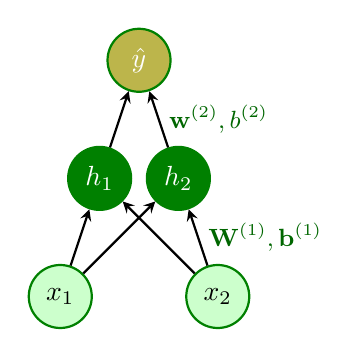
\begin{tikzpicture}[->, >=stealth, node distance=1.5cm, thick]
        % Input nodes
        \node[circle, draw=green!50!black, fill=green!20, minimum size=8mm] (x1) at (0,0) {$x_1$};
        \node[circle, draw=green!50!black, fill=green!20, minimum size=8mm] (x2) at (2,0) {$x_2$};
        
        % Hidden nodes
        \node[circle, draw=green!50!black, fill=green!50!black, text=white, minimum size=8mm] (h1) at (0.5,1.5) {$h_1$};
        \node[circle, draw=green!50!black, fill=green!50!black, text=white, minimum size=8mm] (h2) at (1.5,1.5) {$h_2$};
        
        % Output node
        \node[circle, draw=green!50!black, fill=olive!60, text=white, minimum size=8mm] (y) at (1,3) {$\hat{y}$};
        
        % Edges from input to hidden
        \draw (x1) -- (h1);
        \draw (x1) -- (h2);
        \draw (x2) -- (h1);
        \draw (x2) -- (h2) node[midway, right, font=\small, green!40!black] {$\mathbf{W}^{(1)}, \mathbf{b}^{(1)}$};
        
        % Edges from hidden to output
        \draw (h1) -- (y);
        \draw (h2) -- (y) node[midway, right, font=\small, green!40!black] {$\mathbf{w}^{(2)}, b^{(2)}$};
    \end{tikzpicture}
    \caption{Neural network architecture for the XOR problem.}
    \label{fig:xor_network}
\end{figure}
\noindent
The forward pass is defined as:
\begin{equation*}
    \hat{y} = \mathbf{w}^{(2)\top} \max\left\{0, \mathbf{W}^{(1)\top} \mathbf{x} + \mathbf{b}^{(1)}\right\} + b^{(2)}
\end{equation*}

$$\mathbf{W}^{(1)} = \begin{bmatrix} 1 & 1 \\ 1 & 1 \end{bmatrix}, \quad \mathbf{b}^{(1)} = \begin{bmatrix} 0 \\ -1 \end{bmatrix}, \quad \mathbf{w}^{(2)} = \begin{bmatrix} 1 \\ -2 \end{bmatrix}, \quad b^{(2)} = 0$$

2 inputs, 2 hidden units, 1 output: $4 + 2 + 2 + 1 = 9$ parameters.

\begin{figure}[H]
    \centering
    \[
    \underbrace{
        \begin{bmatrix}
            0 & 0 \\
            0 & 1 \\
            1 & 0 \\
            1 & 1
        \end{bmatrix}
    }_{\mathbf{X}}
    \longrightarrow
    \underbrace{
        \begin{bmatrix}
            0 & 0 \\
            1 & 1 \\
            1 & 1 \\
            2 & 2
        \end{bmatrix}
    }_{\mathbf{X}\mathbf{W}^{(1)}}
    \longrightarrow
    \text{add }\mathbf{b}^{(1)}\text{ to each row}
    \longrightarrow
    \underbrace{
        \begin{bmatrix}
            0 & -1 \\
            1 & 0 \\
            1 & 0 \\
            2 & 1
        \end{bmatrix}
    }_{}
    \longrightarrow
    \underbrace{
        \begin{bmatrix}
            0 & 0 \\
            1 & 0 \\
            1 & 0 \\
            2 & 1
        \end{bmatrix}
    }_{\max\{0, \cdot\}}
    \longrightarrow
    \underbrace{
        \begin{bmatrix}
            0 \\
            1 \\
            1 \\
            0
        \end{bmatrix}
    }_{\times \mathbf{w}^{(2)} = \hat{\mathbf{y}}}
    \]
    \caption{Step-by-step matrix representation of the XOR forward pass for an entire batch.}
    \label{fig:xor_batch_matrices}
\end{figure}
\noindent
In $\mathbf{x}$-space no line separates the classes. In $\mathbf{h}$-space the two positive points 
coincide and a line does:
\begin{equation}
    h_1 - 2h_2 = \frac{1}{2}
\end{equation}
\noindent
The output layer is still a \textbf{linear score}, computed on $\mathbf{h} = \phi(\mathbf{x})$ 
instead of $\mathbf{x}$.
\begin{figure}[H]
    \centering
    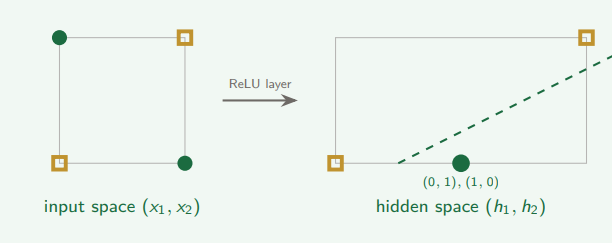
\includegraphics[width=0.7\linewidth]{immagini/xor_nn.png} 
    \caption{Difference between x-space and h-space}
    \label{fig:xor_nn}
\end{figure}